
\subsection{Qubits and Quantum States}
\label{subsec:qubits}

A \textit{qubit} is the fundamental unit of quantum information. Mathematically, a qubit is represented as a normalized vector in a two-dimensional complex Hilbert space, i.e. 
\[
\mathcal{H} = \mathbb{C}^2.
\]
The standard (computational) basis states are defined as
\[
|0\rangle = \begin{pmatrix} 1 \\ 0 \end{pmatrix}, \quad |1\rangle = \begin{pmatrix} 0 \\ 1 \end{pmatrix}.
\]
A general qubit state is given by
\[
|\psi\rangle = \alpha|0\rangle + \beta|1\rangle, \quad \text{with } |\alpha|^2 + |\beta|^2 = 1,
\]
where $\alpha,\beta \in \mathbb{C}$ are the \textit{probability amplitudes}. Note that global phase factors (i.e. multiplication of the state by an overall phase factor $e^{i\gamma}$) are physically irrelevant.

A convenient geometrical representation of qubit states is provided by the \textbf{Bloch sphere}. Any pure qubit state can be written as
\[
|\psi\rangle = \cos\frac{\theta}{2}|0\rangle + e^{i\phi}\sin\frac{\theta}{2}|1\rangle,
\]
with $\theta \in [0, \pi]$ and $\phi \in [0, 2\pi)$. Figure~\ref{fig:bloch_sphere} illustrates this representation.

\begin{figure}[h]
\centering
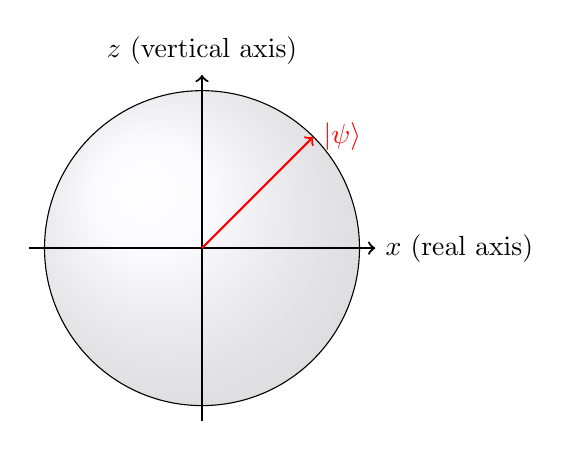
\begin{tikzpicture}[scale=1]
  % Draw sphere outline
  \shade[ball color=blue!10!white,opacity=0.2] (0,0) circle (2cm);
  \draw (0,0) circle (2cm);
  % Axes
  \draw[->, thick] (-2.2,0) -- (2.2,0) node[right] {$x$ (real axis)};
  \draw[->, thick] (0,-2.2) -- (0,2.2) node[above] {$z$ (vertical axis)};
  % Bloch vector
  \draw[->, red, thick] (0,0) -- (1.414,1.414) node[right] {$|\psi\rangle$};
\end{tikzpicture}
\caption{Bloch sphere representation of a qubit.}
\label{fig:bloch_sphere}
\end{figure}

For multi-qubit systems the state space is the tensor product of individual qubit spaces. For example, a two-qubit system is described by
\[
|\psi\rangle = \sum_{i,j \in \{0,1\}} \alpha_{ij}\, |i\rangle \otimes |j\rangle, \quad \sum_{i,j} |\alpha_{ij}|^2 = 1.
\]
This exponential growth in the state space is at the heart of quantum parallelism.
